\section*{Dati e risultati}

Graficando i dati misurati, si ottiene un grafico come quello in Figura \ref{fig:meas}, da cui si può gia stimare
che il punto di inversione è attorno a \SI{6}{\milli\litre}.

Poichè le incertezze sulla conduttanza sono trascurabili rispetto a quelle sul volume, abbiamo eseguito un fit preliminare
solo con le incertezze sulla conduttanza e poi abbiamo trasferito le incertezze dal volume alla conduttanza grazie alla regressione preliminare.
Infine abbiamo eseguito la regressione con i valori trasferiti delle incertezze. 


Abbiamo eseguito il test del chi quadro per verificare che le incertezze fossero corrette.
Per la prima retta abbiamo usato 13 dati, quindi il numero di gradi di libertà è 13 - 2 = 11, poichè
la retta ha 2 parametri. Per la retta che riguarda la salita abbiamo 38 dati e quindi 36 gradi di libertà.
I valori attesi\footnote{L'incertezza sul valore atteso è la radice del valore atteso.} dei $\chi^2$ erano
dunque $11 \pm 3$ e $36 \pm 6$ rispettivamente per la retta in discesa ed in salita.

I valori da noi calcolati sono stati 18 e 3657. In nessuno dei due casi il chi quadro è compatibile con il suo valore atteso.
Abbiamo quindi aggiustato le incertezze (le incertezze corrette sono riportate sul grafico) per far tornare il valore del chi quadro. 

Le incertezze sulla conducibilità corrette sono risultate essere \SI{0.01}{\micro\siemens} per la retta in discesa e di
\SI{0.3}{\micro\siemens} per quella in salita.

È stato quindi rieseguito il fit con le incertezze corrette, per ottenere le incertezze corrette sui parametri delle rette.
I valori definitivi di pendenza ed intercetta sono risultati essere:

\begin{equation*}
    \text{Discesa: }
    \left\{    
    \begin{array}{l}
        m_1 = -0.222 \pm 0.001 ~ \si{\micro\siemens\per\milli\litre} \\
        q_1 = 10.849 \pm 0.005 ~ \si{\micro\siemens} \\
    \end{array}
    \right.
    \qquad
    \qquad
    \text{Salita: }
    \left\{    
        \begin{array}{l}
        m_2 = 1.05 \pm 0.01 ~ \si{\micro\siemens\per\milli\litre} \\
        q_2 = 3.65 \pm 0.15 ~ \si{\micro\siemens} \\
    \end{array}
    \right.
\end{equation*}

L'intersezione tra le due rette indica il volume di soluzione titolante versato per raggiungere
il punto di inversione, e vale:

\begin{equation*}
    p = 5.7 \pm 0.1 ~ \si{\milli\litre}
\end{equation*}

\begin{SCfigure}
    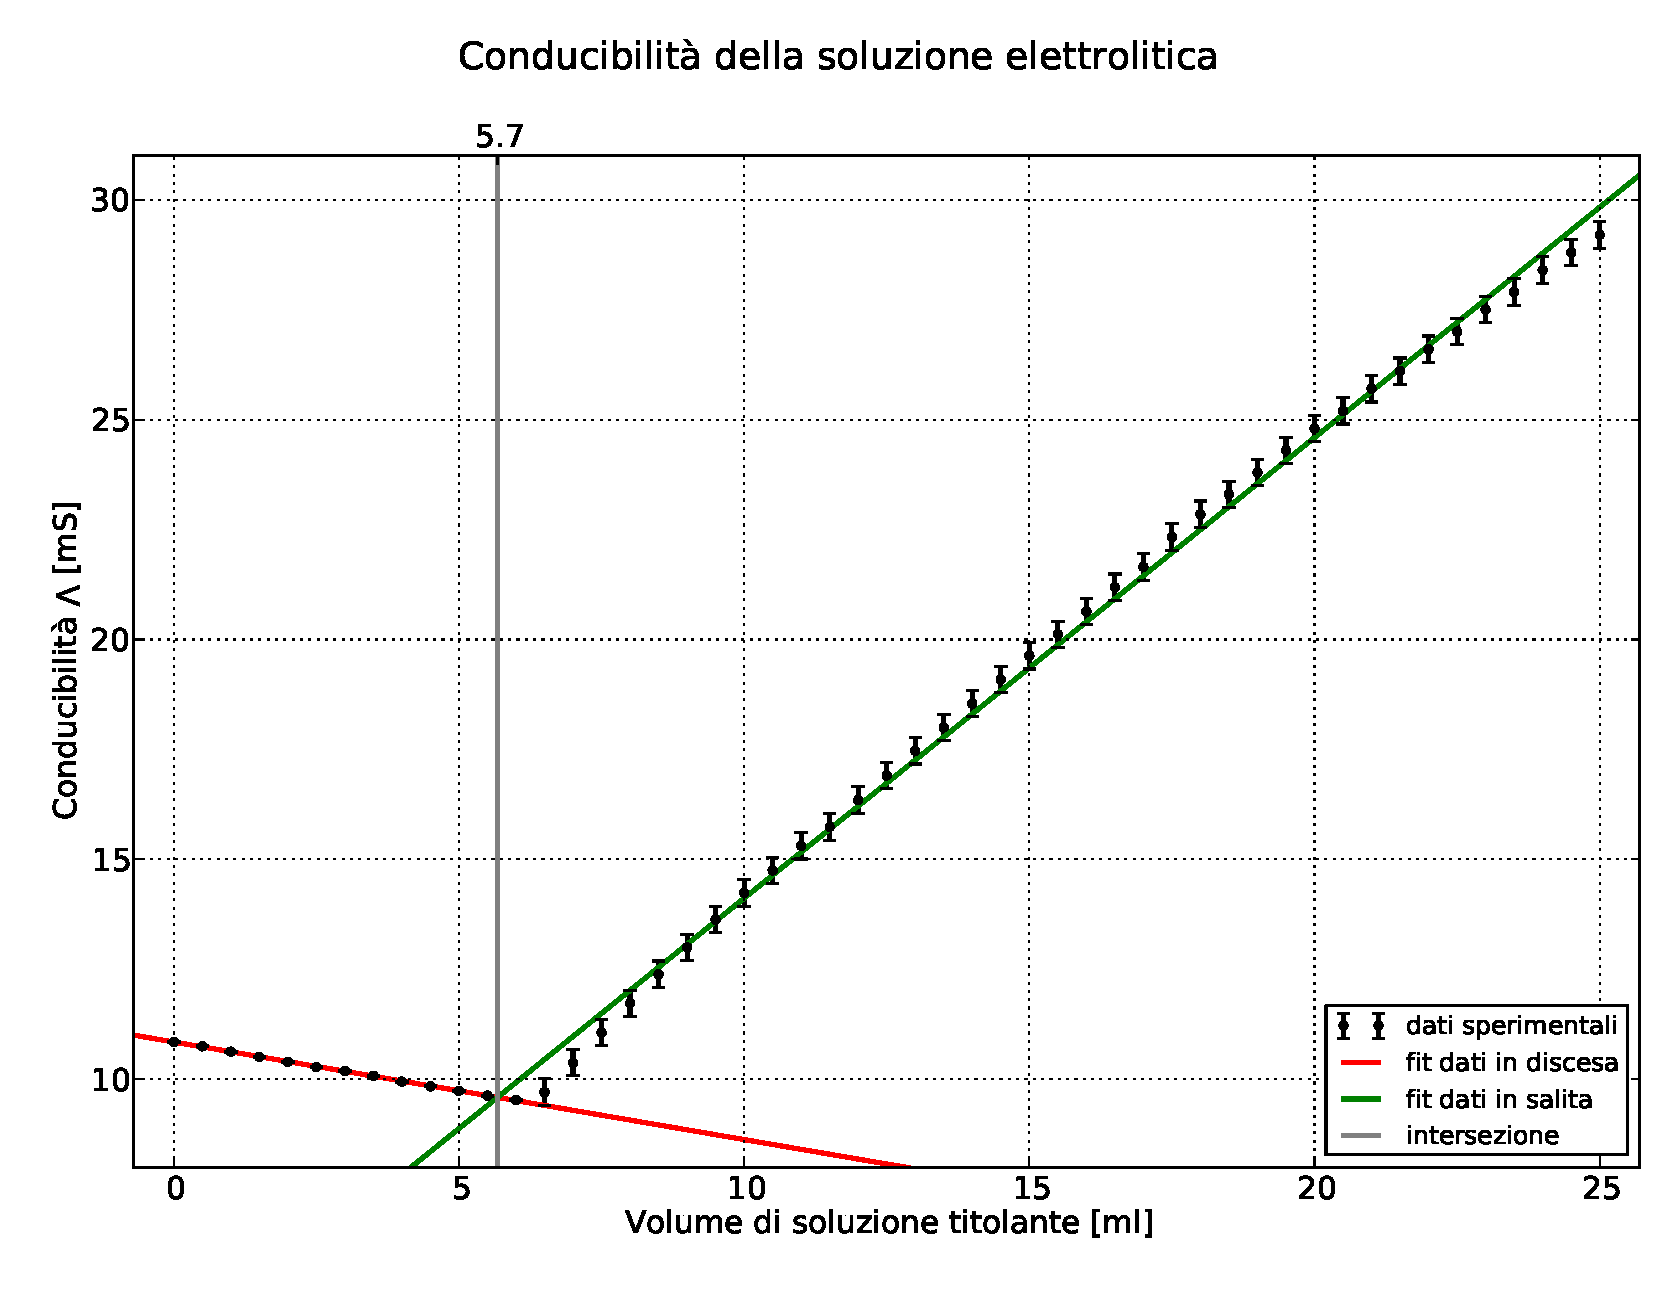
\includegraphics[scale=0.5]{Rette_von_Fitt.pdf}
    \caption{Il grafico illustra i dati  misurati, con relative incertezze, le regressioni lineari
        e il punto di intersezione tra le rette.}
    \label{fig:meas}
\end{SCfigure}
